\documentclass[10pt,a4paper]{article}
\usepackage[utf8]{inputenc}
\usepackage{amsfonts}
\usepackage{graphicx}
\usepackage[letterpaper, margin=1in]{geometry} % page format
\usepackage{indentfirst}
\usepackage{tikz,pgfplots}

\begin{document}

\title{HW3: \\ Autoencoder used on a custom dataset}
\author{Alex Shah}
\date{11/22/17}

\maketitle

\begin{table}[h]
 \caption{2 Layers of Hidden Units Compared to Loss}
 \label{tbl:aTable}
 \begin{center}
  \begin{tabular}{lccccccr}
    \hline 
    Layer1/Layer2 & 1024 & 512 & 256 & 128 & 64 & 32  \\
    \hline
	1024 & X & 1.05 & 1.07 & 1.06 & 1.13 & 1.16 \\
	512  & X & X    & 1.14 & 1.06 & 1.06 & 1.10 \\
	256  & X & X    & X    & 1.15 & X    & X    \\
	128  & X & X    & X    & X    & 1.20 & 1.09 \\
	64   & X & X    & X    & X    & 1.30 & 1.25 \\
	32   & X & X    & X    & X    & X    & 1.59 \\
    \hline 
  \end{tabular}
 \end{center}
\end{table}

\begin{figure}[h]
\begin{center}
	\begin{tikzpicture}
	\begin{axis}[%
	scatter/classes={%
    	a={mark=x,draw=black}}]
	\addplot[scatter,%
	    scatter src=explicit symbolic]%
	table[meta=label] {
	x y label
	512 1.05  a
	256 1.07  a
	128 1.06  a
	64  1.13  a
	32  1.13  a
	    };
	\end{axis}
	\end{tikzpicture}
	\caption{Loss against hidden units 2, when hidden units 1 is 1024}
\end{center}
\end{figure}

	Higher numbers of hidden units were more accurate. Tests where both layers had high numbers of hidden units were more likely to have lower loss and lower error. However in some cases lower pairings of hidden units also had comparable loss and error. For example, the highest pairing of hidden units (1024, 512) had the lowest loss of 1.05. However several pairings of lower hidden units came close. For example (512, 128) had a loss of 1.06. (128, 32) had a loss very close to the lowest at 1.09 and ran much faster than the lowest loss pairings.

\clearpage

\begin{table}[h]
 \caption{2 Layers of Hidden Units Compared to Last Error}
 \label{tbl:aTable}
 \begin{center}
  \begin{tabular}{lccccccr}
    \hline 
    Layer1/Layer2  & 1024 & 512 & 256 & 128 & 64 & 32  \\
    \hline
	1024 & X & 0.6667 & 0.7667 & 0.7833 & 0.6667 & 0.7000 \\
	512  & X & X      & 0.7667 & 0.7667 & 0.7667 & 0.7000 \\
	256  & X & X      & X      & 0.7500 & X      & X      \\
	128  & X & X      & X      & X      & 0.7000 & 0.7000 \\
	64   & X & X      & X      & X      & 0.7167 & 0.6667 \\
	32   & X & X      & X      & X      & X      & 0.7167 \\
    \hline 
  \end{tabular}
 \end{center}
\end{table}

\begin{figure}[h]
\begin{center}
	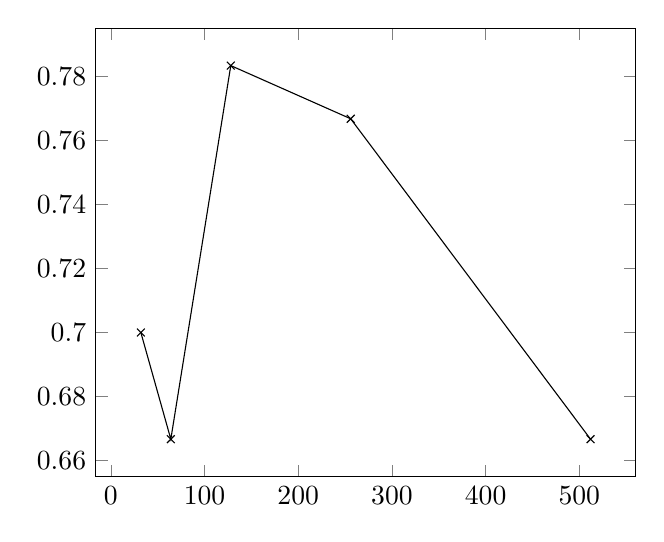
\begin{tikzpicture}
	\begin{axis}[%
	scatter/classes={%
	    a={mark=x,draw=black}}]
	\addplot[scatter,%
	    scatter src=explicit symbolic]%
	table[meta=label] {
	x y label
	512 0.6667  a
	256 0.7667  a
	128 0.7833  a
	64  0.6667  a
	32  0.7000  a
	    };
	\end{axis}
	\end{tikzpicture}
	\caption{Error against hidden units 2, when hidden units 1 is 1024}
	\end{center}
\end{figure}

	Error was a less clear trend, but we can see from Table 2 and Figure 2 that significantly higher and significantly lower numbers of hidden units for the second layer when we look at the first layer, leads to better results. So it seems that the worst accuracy is when the second layer has a medium number of hidden units. It is most likely the case that sample error has formed a coincidental trend here since the number of testing samples is very low and in general the accuracy is very low.

\clearpage

\begin{figure}[h]
\begin{center}
	\begin{tikzpicture}
	\begin{axis}[%
	scatter/classes={%
	    a={mark=x,draw=black}}]
	\addplot[scatter,%
	    scatter src=explicit symbolic]%
	table[meta=label] {
	x y label
	0.01 1.43  a
	0.001 1.12  a
	0.0001 1.05  a
	    };
	\end{axis}
	\end{tikzpicture}
	\caption{Learning Rate Loss, (1024,512)}
	\end{center}
\end{figure}

\begin{figure}[h]
\begin{center}
	\begin{tikzpicture}
	\begin{axis}[%
	scatter/classes={%
	    a={mark=x,draw=black}}]
	\addplot[scatter,%
	    scatter src=explicit symbolic]%
	table[meta=label] {
	x y label
	0.01 0.7333  a
	0.001 0.6333  a
	0.0001  0.6667  a
	    };
	\end{axis}
	\end{tikzpicture}
	\caption{Learning Rate Error (1024,512)}
	\end{center}
\end{figure}

	The next test used the best combination of hidden units (1024, 512) and varied the learning rate. It was clear that smaller learning rates had better (lower) loss and error. A very large learning rate such as 0.1 results in a NaN error and could not finish training. This was an issue with the way the program handled rounding errors and bounds.

\end{document}